\documentclass{beamer}

\usepackage[T1]{fontenc}
\usepackage[utf8]{inputenc}
\usepackage[english]{babel}
\usepackage{amssymb,amsfonts}
\usepackage{lmodern}
\usepackage{tikz}
\usepackage{array}
\usepackage{listings}
\usepackage{subcaption}

\lstset{
    language=C++,        % Language of the code
    basicstyle=\ttfamily,   % Code font style
    keywordstyle=\color{blue}\bfseries,
    stringstyle=\color{red},
    commentstyle=\color{green},
    breaklines=true,        % Auto line breaking
    frame=single           % Add a frame around the code
}


% Use Unipd as theme, with options:
% - pageofpages: define the separation symbol of the footer page of pages (e.g.: of, di, /, default: of)
% - logo: position another logo near the Unipd logo in the title page (e.g. department logo), passing the second logo path as option 
% Use the environment lastframe to add the endframe text
\usetheme[pageofpages=of]{Unipd}

\title{The Smith-Waterman algorithm}
\subtitle{a multithreaded implementation}
\author[Cimino, Gaio, Paolin]{Fabio~Cimino \and Giovanni~Gaio \and Lorenzo~Paolin}

\date{December 16, 2024}

% The next block of commands puts the table of contents at the beginning of each section and highlights the current section
\AtBeginSection[]
{
  \begin{frame}
    \frametitle{Table of Contents}
    \tableofcontents[currentsection]
  \end{frame}
}



\begin{document}

% Make the title page
\frame{\titlepage}

% Insert the general toc
\begin{frame}{Table of Contents}
    \tableofcontents    
\end{frame}




\section{The algorithm}


    \begin{frame}{The problem}
        Genome and protein alignment are fundamental bio-informatics techniques used to compare sequences of DNA, RNA, or proteins to identify regions of similarity.

        \vspace{10pt}
        
        These alignments reveal evolutionary relationships, functional similarities, or conserved regions across species or within different genes and proteins of the same organism.
    \end{frame}

    

    \begin{frame}{The challenge}
        Genomes can consist of billions of base pairs (the human genome has over 3 billion base pairs!).
        
        Aligning such large datasets requires significant computational resources.

        \vspace{10pt}

    \begin{minipage}{0.49\linewidth}
        \begin{figure}
                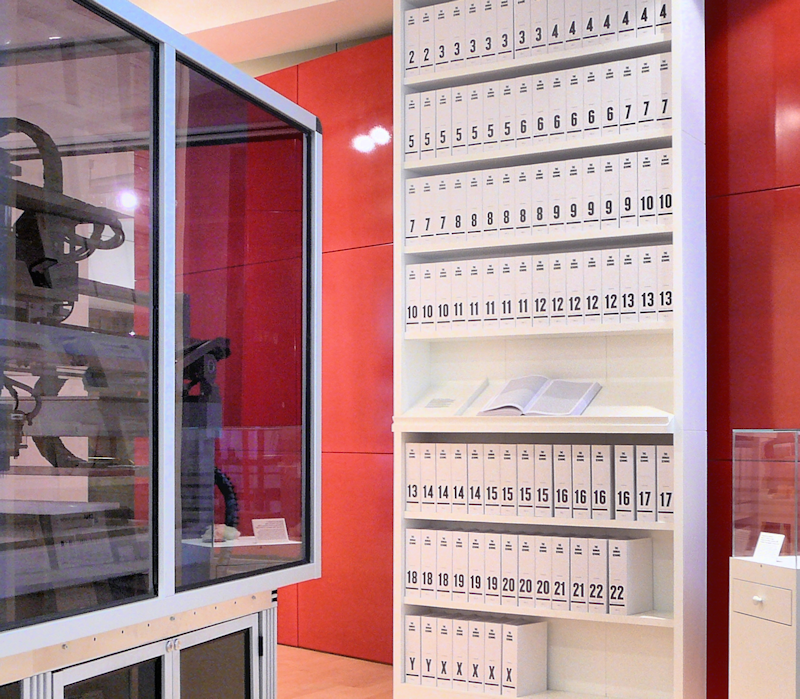
\includegraphics[width=0.8\linewidth]{human_genome_printout.png}
                \caption{Human genome printout}
            \end{figure}
    \end{minipage}
    \begin{minipage}{0.49\linewidth}
        \begin{figure}
            
\includegraphics[width=1\linewidth]{human_genome_book.JPG}
            \caption{Enter Caption}
        \end{figure}
    \end{minipage}
    \end{frame}





    \begin{frame}{How does the algorithm work?}

        The Smith-Waterman algorithm is a dynamic programming algorithm used specifically for local sequence alignment, that is to identify the most similar subsequences between two sequences.

        \vspace{20pt}

        \begin{figure}
            \centering
            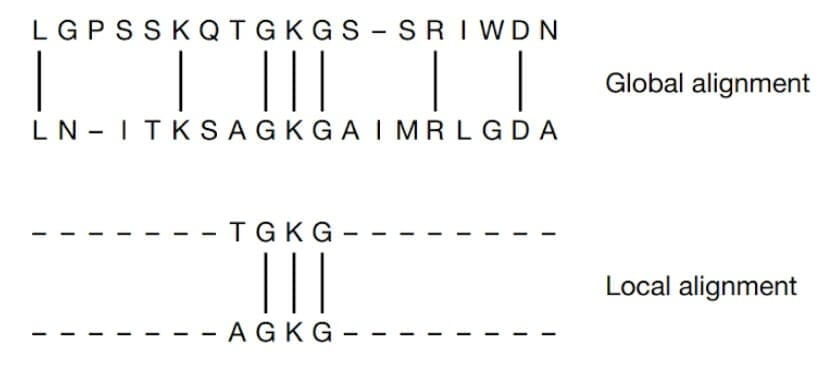
\includegraphics[width=0.5\linewidth]{global_vs_local_alignment.jpg}
        \end{figure}

    \end{frame}



    \begin{frame}{How does the algorithm work?}

        A scoring matrix $H$ is created and filled as follows. The first row and column are initialized to zero.
        \[
            H(i, j) = \max \begin{cases} 
            0 \\
            H(i-1, j-1) + s(i, j) & \text{(match/mismatch)} \\
            H(i-1, j) + g & \text{(deletion)} \\
            H(i, j-1) + g & \text{(insertion)} \\
            \end{cases}
        \]

        \begin{itemize}
            \item $H(i, j)$ is the score at position $(i, j)$,
            \item $s(i, j)$ is the score for a match or mismatch,
            \item $g$ is the penalty for a gap. It can be a function of the gap size. 
        \end{itemize}
        
    \end{frame}

     \begin{frame}{Algorithm data dependencies}

        \begin{minipage}{0.49\linewidth}
            Highlight the dependence of $H(i, j)$ from:
        \begin{itemize}
            \item the previous element along the diagonal $H(i-1, j-1)$,
            \item the previous element along the column $H(i, j-1)$,
            \item the previous element along the row $H(i-1, j)$.
        \end{itemize}

        \vspace{10pt}

        Furthermore, sequences can be insanely huge!
        \end{minipage}
        \begin{minipage}{0.49\linewidth}
            \begin{figure}
            \centering
            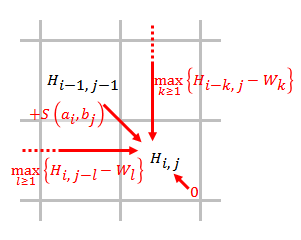
\includegraphics[width=1\linewidth]{algorithm_image.png}
        \end{figure}
        \end{minipage}
        

        

    \end{frame}


\section{The implementation}


   

    \begin{frame}{Implementation challenges}
    \begin{center}
        This is a great and fun challenge!
    \end{center}
        
        \begin{itemize}
            
            \item How do we decompose the problem to handle the dependency chain?
            \item How do we handle synchronization, shared memory access and cache efficiency?
            \item How do we balance the load?
           
        \end{itemize}
    \end{frame}


    

    \begin{frame}{Our solutions}

        We have experimented 3 different approaches using OpenMP:

        \begin{enumerate}
            \item Using locks
            \item Using atomic counters
            \item Using tasks
        \end{enumerate}
        
    \end{frame}



    \begin{frame}{Locks}
            \begin{minipage}{0.3\linewidth}
           \begin{figure}
           \begin{center}
            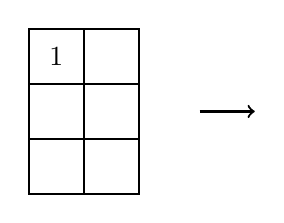
\begin{tikzpicture}[thick,scale=0.7, every node/.style={scale=1}]
                \draw (0,0) -- (0,1) -- (1,1) -- (1,0) -- cycle;
                \draw (1,0) -- (1,1) -- (2,1) -- (2,0) -- cycle;

                \draw (0,1) -- (0,2) -- (1,2) -- (1,1) -- cycle;
                \draw (1,1) -- (1,2) -- (2,2) -- (2,1) -- cycle;

                \draw (0,2) -- (0,3) -- (1,3) -- (1,2) -- cycle;
                \draw (1,2) -- (1,3) -- (2,3) -- (2,2) -- cycle;

                \node at (0.5,2.5) {1};
                \draw[->] (3.1,1.5) -- (4.1, 1.5);
            \end{tikzpicture}
            \end{center}
            \end{figure}
    \end{minipage}
    \hfill
    \begin{minipage}{0.3\linewidth}
           \begin{figure}
           \begin{center}
            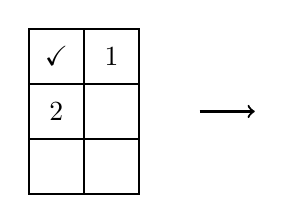
\begin{tikzpicture}[thick,scale=0.7, every node/.style={scale=1}]
                \draw (0,0) -- (0,1) -- (1,1) -- (1,0) -- cycle;
                \draw (1,0) -- (1,1) -- (2,1) -- (2,0) -- cycle;

                \draw (0,1) -- (0,2) -- (1,2) -- (1,1) -- cycle;
                \draw (1,1) -- (1,2) -- (2,2) -- (2,1) -- cycle;

                \draw (0,2) -- (0,3) -- (1,3) -- (1,2) -- cycle;
                \draw (1,2) -- (1,3) -- (2,3) -- (2,2) -- cycle;

                \node at (0.5, 2.5) {\checkmark};
                \node at (1.5,2.5) {1};
                \node at (0.5,1.5) {2};
                \draw[->] (3.1,1.5) -- (4.1, 1.5);
            \end{tikzpicture}
            \end{center}
            \end{figure}
    \end{minipage}
    \hfill
    \begin{minipage}{0.3\linewidth}
           \begin{figure}
           \begin{center}
            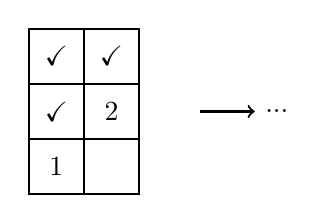
\begin{tikzpicture}[thick,scale=0.7, every node/.style={scale=1}]
                \draw (0,0) -- (0,1) -- (1,1) -- (1,0) -- cycle;
                \draw (1,0) -- (1,1) -- (2,1) -- (2,0) -- cycle;

                \draw (0,1) -- (0,2) -- (1,2) -- (1,1) -- cycle;
                \draw (1,1) -- (1,2) -- (2,2) -- (2,1) -- cycle;

                \draw (0,2) -- (0,3) -- (1,3) -- (1,2) -- cycle;
                \draw (1,2) -- (1,3) -- (2,3) -- (2,2) -- cycle;

                \node at (0.5, 2.5) {\checkmark};
                \node at (1.5, 2.5) {\checkmark};
                \node at (0.5, 1.5) {\checkmark};
                \node at (0.5,0.5) {1};
                \node at (1.5,1.5) {2};
                \draw[->] (3.1,1.5) -- (4.1, 1.5);
                \node at (4.5, 1.5) {...};
            \end{tikzpicture}
            \end{center}
            \end{figure}
    \end{minipage}

        \vspace{10pt}
    
        Divide H in blocks and assign a lock to each. All threads set their own locks.
        
        When a thread wants to work on a block, it sets the lock above it. When it's done, it destroys such lock, and unsets its own. 
    \end{frame}


    \begin{frame}{Atomic counters}

            \begin{minipage}{0.3\linewidth}
           \begin{figure}
           \begin{center}
            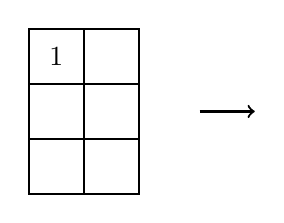
\begin{tikzpicture}[thick,scale=0.7, every node/.style={scale=1}]
                \draw (0,0) -- (0,1) -- (1,1) -- (1,0) -- cycle;
                \draw (1,0) -- (1,1) -- (2,1) -- (2,0) -- cycle;

                \draw (0,1) -- (0,2) -- (1,2) -- (1,1) -- cycle;
                \draw (1,1) -- (1,2) -- (2,2) -- (2,1) -- cycle;

                \draw (0,2) -- (0,3) -- (1,3) -- (1,2) -- cycle;
                \draw (1,2) -- (1,3) -- (2,3) -- (2,2) -- cycle;
                \node at (0.5,2.5) {1};
                \draw[->] (3.1,1.5) -- (4.1, 1.5);
            \end{tikzpicture}
            \end{center}
            \end{figure}
            $C_1 =0, C_2=0$
    \end{minipage}
    \hfill
    \begin{minipage}{0.3\linewidth}
           \begin{figure}
           \begin{center}
            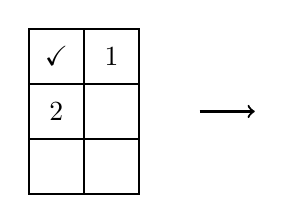
\begin{tikzpicture}[thick,scale=0.7, every node/.style={scale=1}]
                \draw (0,0) -- (0,1) -- (1,1) -- (1,0) -- cycle;
                \draw (1,0) -- (1,1) -- (2,1) -- (2,0) -- cycle;

                \draw (0,1) -- (0,2) -- (1,2) -- (1,1) -- cycle;
                \draw (1,1) -- (1,2) -- (2,2) -- (2,1) -- cycle;

                \draw (0,2) -- (0,3) -- (1,3) -- (1,2) -- cycle;
                \draw (1,2) -- (1,3) -- (2,3) -- (2,2) -- cycle;

                \node at (0.5, 2.5) {\checkmark};
                \node at (1.5,2.5) {1};
                \node at (0.5,1.5) {2};
                \draw[->] (3.1,1.5) -- (4.1, 1.5);
            \end{tikzpicture}
            \end{center}
            \end{figure}
            $C_1 =1, C_2=0$
    \end{minipage}
    \hfill
    \begin{minipage}{0.3\linewidth}
           \begin{figure}
           \begin{center}
            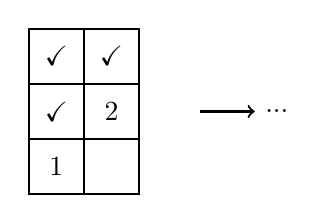
\begin{tikzpicture}[thick,scale=0.7, every node/.style={scale=1}]
                \draw (0,0) -- (0,1) -- (1,1) -- (1,0) -- cycle;
                \draw (1,0) -- (1,1) -- (2,1) -- (2,0) -- cycle;

                \draw (0,1) -- (0,2) -- (1,2) -- (1,1) -- cycle;
                \draw (1,1) -- (1,2) -- (2,2) -- (2,1) -- cycle;

                \draw (0,2) -- (0,3) -- (1,3) -- (1,2) -- cycle;
                \draw (1,2) -- (1,3) -- (2,3) -- (2,2) -- cycle;

               
                \node at (0.5, 2.5) {\checkmark};
                \node at (1.5, 2.5) {\checkmark};
                \node at (0.5, 1.5) {\checkmark};
                \node at (0.5,0.5) {1};
                \node at (1.5,1.5) {2};
                \draw[->] (3.1,1.5) -- (4.1, 1.5);
                \node at (4.5, 1.5) {...};
            \end{tikzpicture}
            \end{center}
            \end{figure}
            $C_1 =2, C_2=1$
    \end{minipage}

        \vspace{10pt}

        Each thread holds a counter of how many blocks it has processed. Thread $i+1$ waits until thread $i$ has processed at least one more block. 

        When threads jump rows the condition is a little different.
        
    \end{frame}



    \begin{frame}{Tasks}
       This is a recursive Divide \& Conquer approach:
       \begin{minipage}{0.55\linewidth}
        \tiny\lstinputlisting{Sections/alg_tasks.cpp}
       \end{minipage}
       \begin{minipage}{0.4\linewidth}
           \begin{figure}
           \begin{center}
            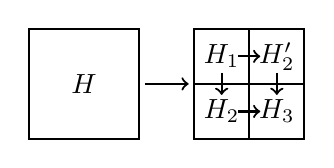
\begin{tikzpicture}[thick,scale=0.7, every node/.style={scale=1}]
                \draw (-1,-1) -- (1,-1) -- (1,1) -- (-1,1) -- cycle;
                \node at (0,0) {$H$};
                \draw[->] (1.1,0) -- (1.9,0);

                \draw (2,0) -- (3,0) -- (3,1) -- (2,1) -- cycle;
                \node at (2.5,+0.5) (A) {$H_1$};
                \draw (2,-1) -- (3,-1) -- (3,0) -- (2,0) -- cycle;
                \node at (2.5,-0.5) (B1) {$H_2$};
                \draw (3,-1) -- (4,-1) -- (4,0) -- (3,0) -- cycle;
                \node at (3.5,+0.5) (B2) {$H_2'$};
                \draw (3,0) -- (4,0) -- (4,1) -- (3,1) -- cycle;
                \node at (3.5,-0.5) (C) {$H_3$};
                \draw[->] (2.5,0.2) -- (2.5,-0.2);
                \draw[->] (2.8,0.5) -- (3.2,0.5);
                %\draw[->] (A) -- (C);
                \draw[->] (3.5,0.2) -- (3.5,-0.2);
                \draw[->] (2.8,-0.5) -- (3.2,-0.5);
            \end{tikzpicture}
            \end{center}
            \end{figure}
        \end{minipage}
    \end{frame}



\section{Performance analysis}

    \begin{frame}{Test setup}

        Dataset generation and characteristics

        Hardware specification
        
    \end{frame}


    \begin{frame}{Performances}

        Execution times, plots

        
        
    \end{frame}


    \begin{frame}{Insights}

        Why these results? Where are the bottlenecks?
        
    \end{frame}



\section{Conclusions}


    \begin{frame}{Moving forward}

        A number of different approaches are possible:
        \begin{enumerate}
            \item Using a similar approach as the ones used, \textbf{MPI} could be well suited to solve this problem: the communication between processes is much smaller than the computation done by each of them.
            \item \textbf{GPUs} could also be very effective, as the computation can proceed row by row and column by column.
            %\item \textbf{Possible improvements}
        \end{enumerate}
    \end{frame}



    \begin{emptyframe}
        Thank you!
    \end{emptyframe}

    \appendix

    \begin{frame}{Backup slide}
        Some additional content
    \end{frame}
    
\end{document}